\documentclass{article}
\usepackage{amsmath}
\usepackage{multicol}
\usepackage[paperwidth=5.5in, paperheight=8.5in, margin=0.2in]{geometry}
\usepackage{pgfplots}
\pgfplotsset{compat=1.18}
\usepackage{graphicx} % Required for inserting images
\usepackage{tgadventor}
\renewcommand*\familydefault{\sfdefault} %% Only if the base font of the document is to be sans serif
\usepackage[T1]{fontenc}

\pgfplotsset{
    every axis/.append style={
        scale only axis,
        width=0.75\textwidth,
        xtick={0,0.05,0.1},
    }
}
\begin{document}
\begin{align*}
f(x)=
\begin{cases}
2x -1 & \text{ if } -4 \leq x \leq -1 \\ 
2x & \text{ if } -1 < x \leq 4
\end{cases}
\end{align*}

brash
\vspace{2in}
\hrule
\vspace{0.5in}

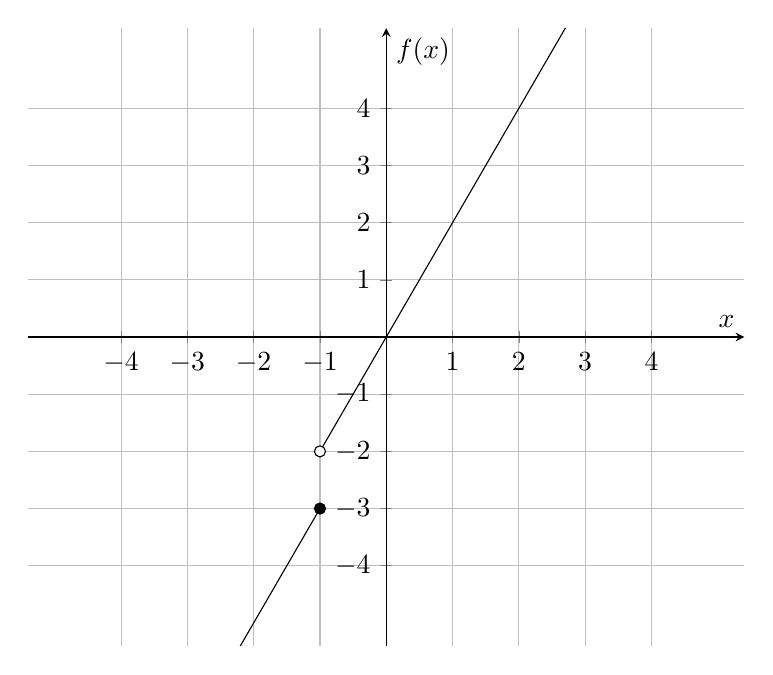
\begin{tikzpicture}
\begin{axis}[axis lines = middle,
            xlabel = $x$, ylabel = $f(x)$,
            domain=-4:4,
            samples=200,
            ymin=-4.5, ymax=4.5,
            xmin=-4.5, xmax=4.5,
            grid=both,
            xtick={-4,-3,-2,-1,1,2,3,4},
            ytick={-4,-3,-2,-1,1,2,3,4},
            enlargelimits=true]
\addplot[domain=-4:-1]{2*x^1-1*x^0};
\addplot[domain=-1:4]{2*x^1};
% Open circles at discontinuities
\addplot[only marks, mark=*, fill=black] coordinates{(-4,-9)};
\addplot[only marks, mark=*, fill=black] coordinates{(-1,-3)};
\addplot[only marks, mark=*, fill=white] coordinates{(-1,-2)};
\addplot[only marks, mark=*, fill=black] coordinates{(4,8)};
\end{axis}
\end{tikzpicture}

\vspace{2ex}
Liam

\pagebreak
\begin{align*}
f(x)=
\begin{cases}
2 & \text{ if } -10 \leq x < -2 \\ 
-x & \text{ if } -2 \leq x \leq 0 \\ 
-2 & \text{ if } 0 < x \leq 10
\end{cases}
\end{align*}

brittle
\vspace{2in}
\hrule
\vspace{0.5in}

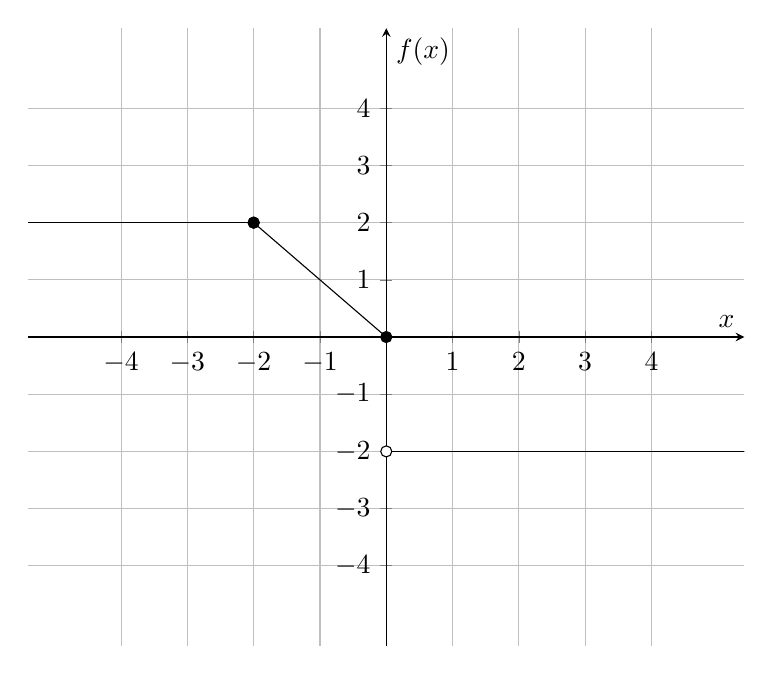
\begin{tikzpicture}
\begin{axis}[axis lines = middle,
            xlabel = $x$, ylabel = $f(x)$,
            domain=-4:4,
            samples=200,
            ymin=-4.5, ymax=4.5,
            xmin=-4.5, xmax=4.5,
            grid=both,
            xtick={-4,-3,-2,-1,1,2,3,4},
            ytick={-4,-3,-2,-1,1,2,3,4},
            enlargelimits=true]
\addplot[domain=-10:-2]{2*x^0};
\addplot[domain=-2:0]{-1*x^1};
\addplot[domain=0:10]{-2*x^0};
% Open circles at discontinuities
\addplot[only marks, mark=*, fill=black] coordinates{(-10,2)};
\addplot[only marks, mark=*, fill=white] coordinates{(-2,2)};
\addplot[only marks, mark=*, fill=black] coordinates{(-2,2)};
\addplot[only marks, mark=*, fill=black] coordinates{(0,0)};
\addplot[only marks, mark=*, fill=white] coordinates{(0,-2)};
\addplot[only marks, mark=*, fill=black] coordinates{(10,-2)};
\end{axis}
\end{tikzpicture}

\vspace{2ex}
Olivia

\pagebreak
\begin{center}
\Large Answer Key
\end{center}
\begin{itemize}
\item brash : Liam
\end{itemize}
\begin{itemize}
\item brittle : Olivia
\end{itemize}
\end{document}

